\documentclass[a5paper,12pt,openany]{scrbook}
\usepackage[papersize={148.5mm,215mm},twoside,bindingoffset=0.5cm,hmargin={1cm,1cm},
				vmargin={2cm,2cm},footskip=1.1cm,driver=dvipdfm]{geometry}

\usepackage{graphicx}
\usepackage{palatino}
\usepackage{microtype}

\makeatletter
\newcommand{\judul}[1]{%
  {\parindent \z@ \centering \normalfont
    \interlinepenalty\@M \Large \bfseries #1\par\nobreak \vskip 20\p@ }}
\newcommand{\subjudul}[1]{%
  {\parindent \z@ \normalfont
    \interlinepenalty\@M \bfseries #1\par\nobreak \vskip 20\p@ }}
\newcommand{\lagu}[1]{%
  {\parindent \z@ \normalfont
    \interlinepenalty\@M \bfseries \emph{#1}\par\nobreak \vskip 20\p@ }}

\renewenvironment{description}
               {\list{}{\labelwidth\z@ \itemindent-\leftmargin
                        \let\makelabel\descriptionlabel}}
               {\endlist}
\renewcommand*\descriptionlabel[1]{\hspace\labelsep 
                                \normalfont\bfseries #1 }
    

\makeatother

\newcommand{\BU}[1]{\begin{itemize} \item[U:] #1 \end{itemize}}
\newcommand{\BI}[1]{\begin{itemize} \item[P:] #1 \end{itemize}}
\newcommand{\BP}[1]{\begin{itemize} \item[P:] #1 \end{itemize}}
% \newcommand{\BL}[1]{\begin{itemize} \item[Wawan:] #1 \end{itemize}}
% \newcommand{\BW}[1]{\begin{itemize} \item[Novi:] #1 \end{itemize}}
% \newcommand{\BMP}[1]{\begin{itemize} \item[W+N:] #1 \end{itemize}}
% \newcommand{\BS}[1]{\begin{itemize} \item[Saksi:] #1 \end{itemize}}

\usepackage[bahasa]{babel}
\selectlanguage{bahasa}

\title{Menyongsong\\ Pesta Keluarga Kudus}
\date{28 Desember 2019}
\author{Keluarga besar trah VF Parlan\\Pundung\\~~\\~~\\}
\begin{document}
\maketitle
\thispagestyle{empty}
~
\newpage
\judul{PEMBUKA}

\lagu{Lagu pembuka}
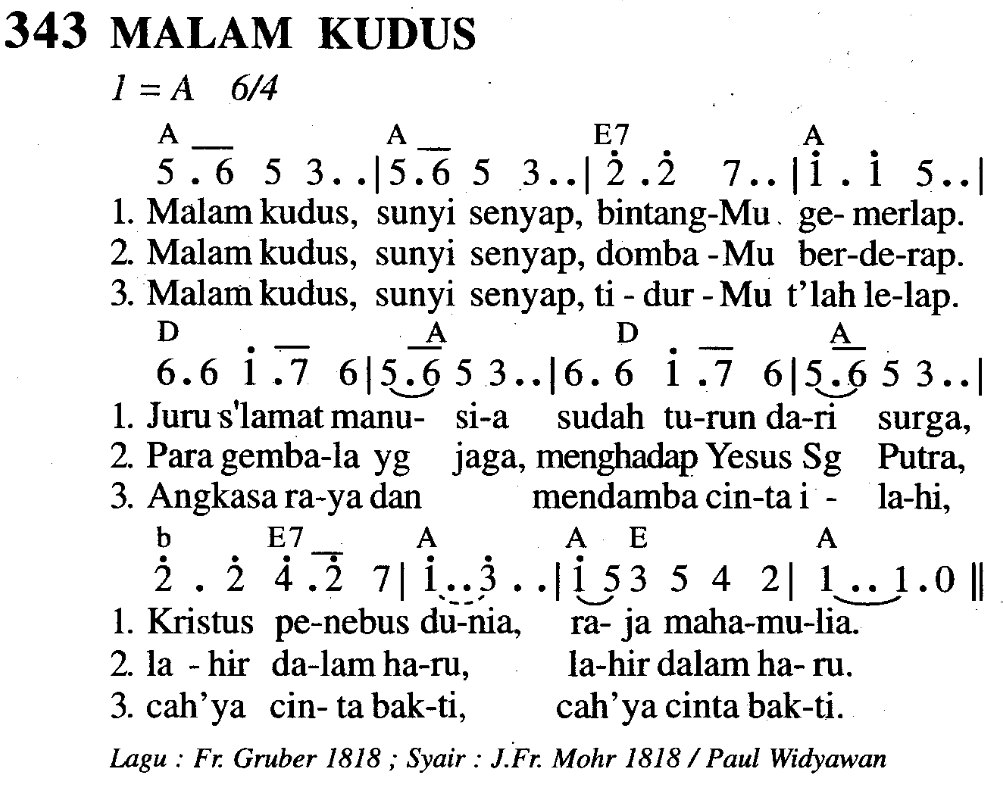
\includegraphics[scale=0.3]{mb343-malam-kudus.png}

\subjudul{Tanda Salib}
\BI{Dalam nama Bapa dan Putera dan Roh Kudus}
\BU{Amin}

\subjudul{Salam Pembukaan}
\BI{Rahmat Tuhan kita Yesus Kristus, cinta kasih Allah, dan persekutuan Roh Kudus beserta kita}
\BU{Sekarang dan selama-lamanya}

\subjudul{Pengantar}
\BI{Bapak, Ibu, dan Saudara-saudara, seperti kita tahu hari ini adalah \textit{Pesta Keluarga Kudus Nasareth}. Kita mempunyai teladan sebuah keluarga yang sederhana dan taat.

Keluarga kita sudah berjalan beberapa lama. Suatu perjalanan ziarah yang penuh dengan suka dan duka, dan kenangan. Suatu perjalanan yang tidak pernah lepas dari berkat dan rahmat Tuhan. Berkat dan rahmat itu sungguh-sungguh nyata dan dirayakan oleh keluarga kita terutama melalui segala kebaikan yang telah kita terima dari orang-orang di sekitar kita.

Ibadat syukur ini sebagai ungkapan terima kasih atas segala kebaikan yang senantiasa mengalir di dalam keluarga kita.}

\subjudul{Tobat}
\BI{Marilah kita hening sejenak untuk mempersiapkan diri dalam ibadat ini sambil menyadari bahwa kita sering melupakan kebaikan Tuhan dan enggan mewartakan dan mewujudkan kebaikan tersebut melalui pikiran, perkataan, dan perbuatan kita.}

\BI{Saya mengaku}

\BU{Kepada Allah yang Maha Kuasa dan kepada saudara sekalian bahwa saya telah berdosa dengan pikiran dan perkataan, dengan perbuatan dan kelalaian. Saya berdosa, saya berdosa, saya sungguh berdosa. Oleh sebab itu saya mohon kepada Santa Perawan Maria, kepada Para Malaikat dan orang kudus dan kepada saudara sekalian, supaya mendoakan saya kepada Allah Tuhan kita.}

\BI{Semoga Allah Yang Maha Kuasa mengasihi kita, mengampuni dosa kita dan menghantar kita ke hidup yang kekal.}

\BU{Amin}

\lagu{Tuhan Kasihanilah Kami}

\subjudul{Doa Pembuka}

\BI{Marilah kita berdoa,

Ya Allah, Engkau berkenan memberikan kepada kami Keluarga Kudus sebagai teladan yang unggul. Semoga kami meneladaninya dalam keutamaan hidup berkeluarga dan dalam ikatan cinta agar kami layak menikmati dengan penuh sukacita anugerah hidup abadi di dalam rumah-Mu.

Semoga keluarga besar ini tetap terus bercermin pada segala kebaikan yang senantiasa mengalir dari orang-orang disekitar mereka. Dengan demikian keluarga besar ini senantiasa hidup dalam kedamaian, kerukunan, dan kesederhanaan, demi Yesus Kristus Putera-Mu, Tuhan dan Pengantara kami yang hidup bersama Dikau dalam persekutuan Roh Kudus kini dan sepanjang masa.}

\BU{Amin}

\judul{SABDA}

\subjudul{Bacaan pertama: Ibrani 11:8,11-12,17-19}

\BP{\emph{Pembacaan dari Surat Rasul Paulus kepada Umat Ibrani.}

Karena iman Abraham taat, ketika ia dipanggil untuk berangkat ke negeri yang akan diterimanya menjadi milik pusakanya, lalu ia berangkat dengan tidak mengetahui tempat yang ia tujui.

Karena iman ia juga dan Sara beroleh kekuatan untuk menurunkan anak cucu, walaupun usianya sudah lewat, karena ia menganggap Dia, yang memberikan janji itu setia.

Itulah sebabnya, maka dari satu orang, malahan orang yang telah mati pucuk, terpancar keturunan besar, seperti bintang di langit dan seperti pasir di tepi laut, yang tidak terhitung banyaknya.

Karena iman maka Abraham, tatkala ia dicobai, mempersembahkan Ishak. Ia, yang telah menerima janji itu, rela mempersembahkan anaknya yang tunggal, walaupun kepadanya telah dikatakan: "Keturunan yang berasal dari Ishaklah yang akan disebut keturunanmu."
Karena ia berpikir, bahwa Allah berkuasa membangkitkan orang-orang sekalipun dari antara orang mati. Dan dari sana ia seakan-akan telah menerimanya kembali.

Demikianlah Sabda Tuhan
}

\BU{Syukur kepada Allah.}

\lagu{Lagu tanggapan sabda}

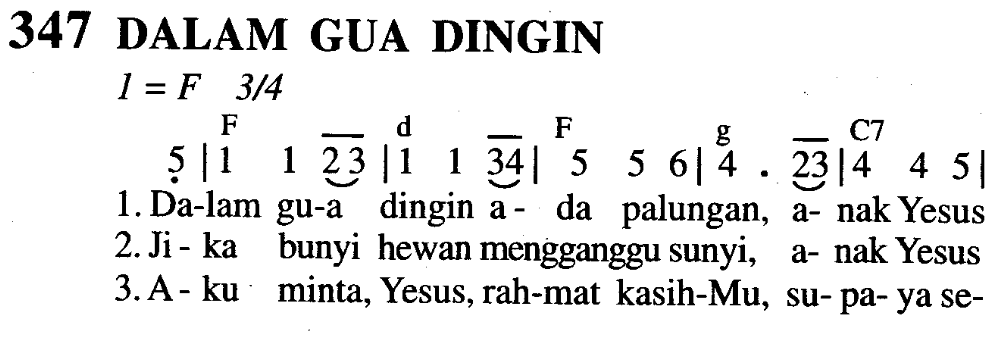
\includegraphics[scale=0.3]{mb347-dalam-gua-dingin-a.png}

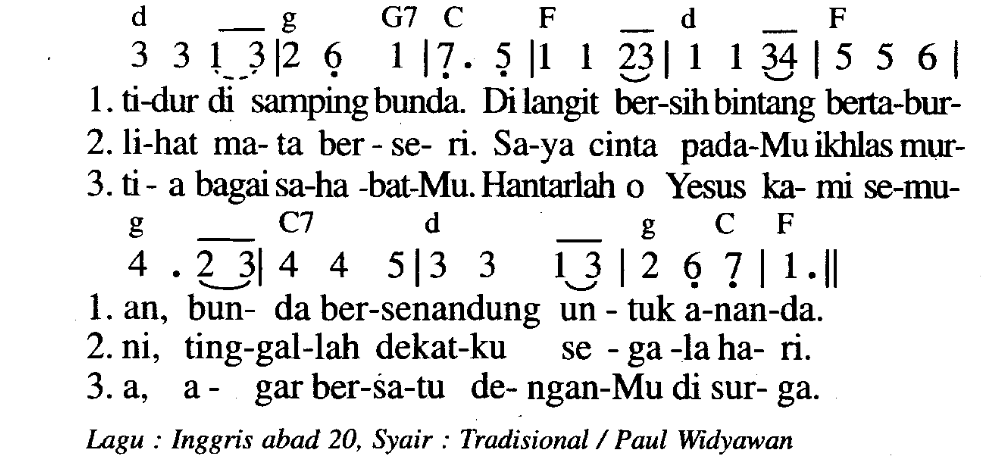
\includegraphics[scale=0.3]{mb347-dalam-gua-dingin-b.png}

\subjudul{Bacaan Injil:  Lukas 2:22-40}

\BI{Semoga Tuhan beserta kita}

\BU{Sekarang dan selama-lamanya}

\BI{Inilah Injil Yesus Kristus menurut Santo Lukas}

\BU{Dimuliakanlah Tuhan}

\BI{Dan ketika genap waktu pentahiran, menurut hukum Taurat Musa, mereka membawa Dia ke Yerusalem untuk menyerahkan-Nya kepada Tuhan,
seperti ada tertulis dalam hukum Tuhan: "Semua anak laki-laki sulung harus dikuduskan bagi Allah",
dan untuk mempersembahkan korban menurut apa yang difirmankan dalam hukum Tuhan, yaitu sepasang burung tekukur atau dua ekor anak burung merpati.

Adalah di Yerusalem seorang bernama Simeon. Ia seorang yang benar dan saleh yang menantikan penghiburan bagi Israel. Roh Kudus ada di atasnya,
dan kepadanya telah dinyatakan oleh Roh Kudus, bahwa ia tidak akan mati sebelum ia melihat Mesias, yaitu Dia yang diurapi Tuhan.

Ia datang ke Bait Allah oleh Roh Kudus. Ketika Yesus, Anak itu, dibawa masuk oleh orang tua-Nya untuk melakukan kepada-Nya apa yang ditentukan hukum Taurat,
ia menyambut Anak itu dan menatang-Nya sambil memuji Allah, katanya:
"Sekarang, Tuhan, biarkanlah hamba-Mu ini pergi dalam damai sejahtera, sesuai dengan firman-Mu,
sebab mataku telah melihat keselamatan yang dari pada-Mu,
yang telah Engkau sediakan di hadapan segala bangsa,
yaitu terang yang menjadi penyataan bagi bangsa-bangsa lain dan menjadi kemuliaan bagi umat-Mu, Israel."
Dan bapa serta ibu-Nya amat heran akan segala apa yang dikatakan tentang Dia.

Lalu Simeon memberkati mereka dan berkata kepada Maria, ibu Anak itu: "Sesungguhnya Anak ini ditentukan untuk menjatuhkan atau membangkitkan banyak orang di Israel dan untuk menjadi suatu tanda yang menimbulkan perbantahan
'dan suatu pedang akan menembus jiwamu sendiri', supaya menjadi nyata pikiran hati banyak orang."

Lagipula di situ ada Hana, seorang nabi perempuan, anak Fanuel dari suku Asyer. Ia sudah sangat lanjut umurnya. 
Sesudah kawin ia hidup tujuh tahun lamanya bersama suaminya,
dan sekarang ia janda dan berumur delapan puluh empat tahun. Ia tidak pernah meninggalkan Bait Allah dan siang malam beribadah dengan berpuasa dan berdoa.
Dan pada ketika itu juga datanglah ia ke situ dan mengucap syukur kepada Allah dan berbicara tentang Anak itu kepada semua orang yang menantikan kelepasan untuk Yerusalem.

Dan setelah selesai semua yang harus dilakukan menurut hukum Tuhan, kembalilah mereka ke kota kediamannya, yaitu kota Nazaret di Galilea.
Anak itu bertambah besar dan menjadi kuat, penuh hikmat, dan kasih karunia Allah ada pada-Nya.

Demikianlah Injil Tuhan
}

\BU{Terpujilah Kristus}

\subjudul{Homili}


\subjudul{Doa Umat}

\BI{Marilah kita sebagai satu keluarga besar berdoa kepada Allah Bapa kita bersama:}

\BP{Bagi Gereja Kristus: Semoga Allah Bapa memperkenankan Gereja berkembang menjadi keluarga besar, di mana cinta kasih dan hormat terhadap tanggung jawab menjadi ciri-cirinya yang khas. Marilah kita mohon, \dots\dots}

\BU{Tuhan, dengarkanlah umat-Mu.} 

\BP{Bagi para bapak dan ibu: Semoga Allah Bapa mendampingi para bapak dan ibu, agar mereka dalam kesulitan tetap tabah bertahan, karena yakin bahwa cinta kasihnya yang tanpa pamrih menjadi jaminan pendidikan anak-anak mereka. Marilah kita mohon,...}

\BU{Tuhan, dengarkanlah umat-Mu.}

\BP{Bagi kaum muda kita: Semoga Allah Bapa menyadarkan kaum muda kami bahwa hari depan mereka harus mereka bangun dengan kebebasan, tetapi penuh tanggung jawab. Marilah kita mohon, \dots\dots}

\BU{Tuhan, dengarkanlah umat-Mu.}

\BP{Bagi keluarga-keluarga kita masing-masing: Semoga Allah Bapa memberkati keluarga-keluarga kita dalam usaha untuk menciptakan suasana akrab terbuka dan penuh cinta kasih berdasarkan iman yang mendalam. Marilah kita mohon,....}

\BU{Tuhan, dengarkanlah umat-Mu.}

\BI{Allah Bapa kami yang Mahabaik, demikianlah permohonan kami, sebagai ungkapan cita-cita kami akan dunia baru yang lebih baik, di mana kami hidup dengan gembira dan penuh gairah, sekarang dan selama-lamanya.}

\BU{Amin.} 


\BI{Pada Pesta Keluarga Kudus di Nasaret ini, marilah berdoa kepada Allah Bapa kita sebagai satu keluarga anak Allah}

\BP{\textbf{Doa suami istri (\textit{oleh Bapak-Ibu})}

Allah, sumber cinta sejati, Engkau telah mempersatukan kami dalam ikatan perkawinan yang suci. Kami bersyukur atas segala pengalaman selama perjalanan perkawinan kami: atas segala suka dan duka; atas kebahagiaan dan penderitaan; atas untung dan malang; terlebih atas rahmat kesetiaan yang telah memungkinkan kami berdua berpegang teguh pada ikrar perkawinan kami: berpadu dalam cinta.

Kami bersyukur pula atas anak-anak yang Kau percayakan kepada kami. Bantulah kami agar selalu setia satu sama lain; tak jemu-jemu mengusahakan kebahagiaan pasangan; tak enggan untuk saling berkorban; bersikap jujur, dan terbuka demi keutuhan keluarga; saling menopang bila menanggung beban; dan siap saling mengampuni bila suatu saat kami jatuh.

Semoga karena berkat-Mu kami saling menguatkan dalam menghadapi tantangan dan godaan yang mangancam keutuhan keluarga kami. Semoga dari hari ke hari perpaduan kasih kami semakin kuat, dan perkawinan kami sungguh menjadi sakramen kasih Kristus terhadap Gereja. Dan kelak, apabila tugas kami di dunia telah selesai, perkenankanlah kami berdua menikmati kebahagiaan abadi bersama-Mu.

Nyalakanlah selalu api kasih yang mengobarkan semangat kami saat mengikrarkan janji perkawinan. Kuatkanlah kami untuk selalu mengutamakan kebahagiaan keluarga.
Kami unjukkan doa ini kepada-Mu, ya Bapa, demi Yesus Kristus junjungan dan teladan kami, kini dan sepanjang masa. Amin}


\BP{\textbf{Doa untuk orangtua (\textit{oleh anak-anak})}

Ya Allah, Bapa yang penuh kasih sayang, kami bersyukur kepada-Mu atas orangtua kami. Lewat mereka Engkau telah menciptakan kami. Melalui kasih sayang mereka, Engkau menyayangi kami. Mereka mendidik, mendampingi, dan menuntun kami. Mereka membesarkan kami dan menjadi sahabat kami.
Berkatilah mereka senantiasa. Berilah mereka kesabaran. Terangilah akal budi mereka supaya mereka selalu bertindak bijaksana. Berilah mereka kesehatan agar tetap mampu menjalankan tugas mereka sebagai pembina keluarga. Berilah rezeki secukupnya untuk kami semua; dan hindarkanlah orangtua kami dari marabahaya. Sempurnakanlah kasih mereka satu sama lain, sehingga mereka dapat menjaga kelestarian perkawinan, dan tetap setia pada janji perkawinan mereka.

Semoga mereka dapat menjalankan tugas dengan baik bagi Gereja, masyarakat, dan keluarga. Buatlah keluarga kami menjadi Gereja kecil yang selalu mengasihi-Mu dan mengasihi Yesus, Putra-Mu.
Kami mohon pula berkat-Mu untuk semua orangtua, yang dengan rela dan penuh tanggung jawab telah menjalankan tugas selaku orangtua atas anak-anak mereka. Semoga pengorbanan mereka tidak sia-sia. Bila mereka menghadapi kesulitan dan tantangan, sudilah Engkau menunjukan jalan keluar yang diperlukan. Jangan biarkan mereka merana karena kegetiran hidup ini.

Kami berdoa pula bagi para orangtua yang sering dilupakan oleh anak-anak mereka. Sudilah Engkau menghibur dan menguatkan hati mereka. Teristimewa kami berdoa bagi para orangtua yang merasa gagal dalam membangun keluarga dan mendidik anak-anak. Semoga kepedihan ini tidak membuat mereka putus asa, tetapi semakin menyadarkan mereka untuk senantiasa bersandar pada-Mu.

Bapa, semua permohonan ini kami unjukan kepada-Mu demi Yesus Kristus Putra-Mu, yang menjadi teladan kami dalam menghormati dan mengasihi orangtua. Dialah pengantara kami untuk selama-lamanya. Amin
}
\normalsize

\BP{\textbf{Doa untuk anak (\textit{oleh orangtua})}

Ya Allah yang mahakuasa, Engkau telah menciptakan anak kami menurut gambar dan citra-Mu sendiri. Terima kasih atas martabat luhur yang Kau berikan kepada mereka, dan terima kasih bahwa kami boleh menjadi alat-Mu untuk mengasuh mereka. Ya Bapa, kami serahkan mereka kepada kebijaksanaan-Mu. Jagailah mereka agar semakin menyerupai Yesus, yang semakin besar semakin bertambah pula hikmat-Nya, semakin berkenan pada-Mu dan pada sesama. Tuntunlah mereka agar tetap setia pada panggilannya selaku orang kristen; bantulah mereka menekuni tugas mereka dengan penuh semangat dan tanggung jawab; lindungilah mereka dari segala marabahaya. Terangilah mereka dalam memilih jalan hidup yang selaras dengan kehendak-Mu. Semoga mereka setia kepada jalan hidup yang telah mereka pilih, dan dapat menjadikan panggilannya sebagai sarana pengabdian kepada masyarakat, kepada jemaat, dan kepada-Mu sendiri. Bila mereka mengalami kesulitan, sudilah Engkau selalu mandampingi, jangan sampai mereka lemah semangat apa lagi putus asa.

Kami mohon berkat-Mu bagi anak-anak yang terpaksa berpisah dari orangtua, lalu mengikuti orangtua asuh; semoga dalam keluarga baru ini pun mereka mendapatkan kasih yang mereka perlukan. Kami berdoa pula bagi anak-anak yang karena berbagai sebab tidak memperoleh bimbingan selayaknya. Peliharalah mereka, dan bantulah kami agar dapat turut mendampingi mereka menyiapkan masa depan.
Terlebih kami berdoa bagi anak-anak yang terlantar dan gagal. Sudilah Engkau membangkitkan kasih dalam diri setiap orang untuk membantu mereka membina masa depan yang penuh harapan.
Permohonan ini kami serahkan kepada kebijaksanaan-Mu, Bapa, sebab Engkaulah Bapa sekalian anak, demi Kristus, Tuhan kami. Amin}

\BP{\textbf{Doa Penyerahan diri kepada Keluarga Kudus Nazaret (\textit{semua})}

Keluarga Kudus, Teladan dan Pelindung segenap keluarga Kristiani,
di bawah naunganmu kami serahkan keluarga kami.

Bila hidupmu kami renungkan kembali,
tergeraklah hati kami untuk menimba semangatmu.

Bapa Yusuf dan Bunda Maria, sejak terbentuknya keluargamu,
nyatalah kesediaan untuk saling menerima dan mendukung
yang ditopang oleh tanggapanmu atas panggilan Allah.

Seluruh perjuangan hidupmu diwarnai oleh iman, kelutusan dan kerendahan hati,
ikut membantu menangkap kehendak Allah
yang terwujud dalam tanggung jawab dan cintamu kepada Yesus.

Dalam hidup tersembunyi di Nazaret, Bapa dan Bunda bekerja keras
membanting tulang dan hidup sederhana.

Asuhlah kami untuk menyambut kehadiran Yesus di antara kami;
menciptakan keheningan di tengah kesibukan,
berani menyimpan sabda-Nya di dalam hati
sebagai pegangan hidup persaudaraan sehari-hari;
mau bekerjasama, saling membantu dan meneguhkan dan bukan menambah penderitaan.

Tuhan Yesus, semoga berkat kedudukan-Mu sebagai titik temu dalam keluarga kami,
kami bersedia meluangkan waktu untuk saling bertemu,
menjalin relasi manusiawi yang matang,
sehingga rumah kami terasa mengerasankan aman tenteram dan penuh kasih sayang.

Ajarilah kami untuk mengambil sikap yang tepat
antara tugas dan kepentingan pribadi maupun keluarga.

Keluarga Kudus Nazaret, kami percaya bahwa dengan menimba semangat hidupmu
semakin terpancarlah dari hidup kami
kesaksian dan pewartaan mengenai kasih sebagai pengikat
yang mempersatukan dan menyempurnakan.

Terpujilah nama Yesus, Maria dan Yusuf,
sekarang dan selama-lamanya.

Amin.}

\subjudul{Bapa kami}

\subjudul{Penutup}
\BI{Marilah kita berdoa,

Bapa yang Mahapenyayang, Engkau sudah menyegarkan kami dengan sabdaMu. Semoga kami senantiasa mengikuti teladan Keluarga Kudus agar sesudah suka duka dunia ini, kamu masuk dalam persekutuan abadi bersama mereka.
Demi Kristus, Tuhan dan Pengantara kami. Kini, selalu, dan sepanjang segala abad.}

\BU{Amin}

\BI{Semoga Tuhan beserta kita}
\BU{Sekarang dan selama-lamanya}
\BI{Semoga keluarga kita semua senantiasa dibimbing dan dilindungi dengan limpahan berkat dari Allah Yang Maha Baik. ($\dagger$) Dalam Nama Bapa, Putra, dan Roh Kudus}
\BU{Amin}
\BI{Dengan demikian ibadat hari ini telah selesai.}
\BU{Syukur kepada Allah.}

\lagu{Lagu penutup}

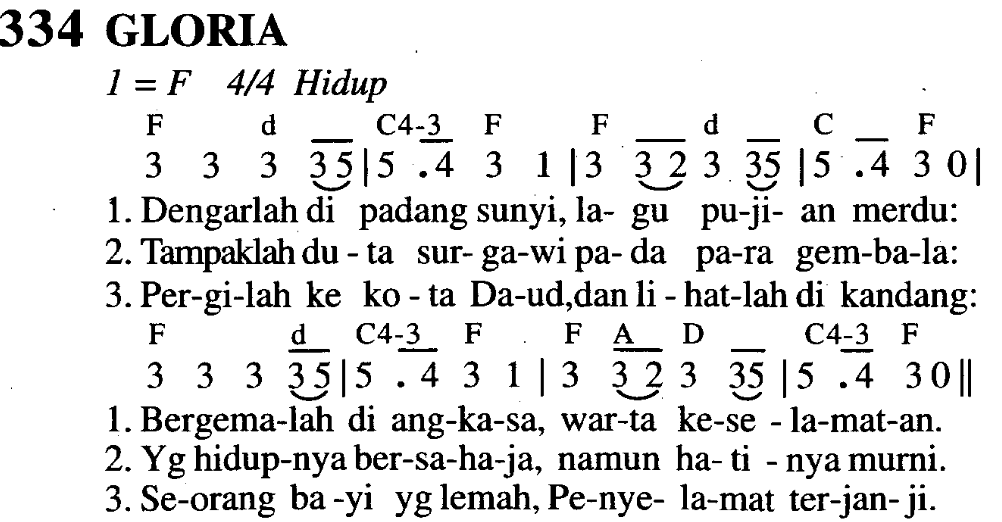
\includegraphics[scale=0.3]{mb334-gloria-a.png}

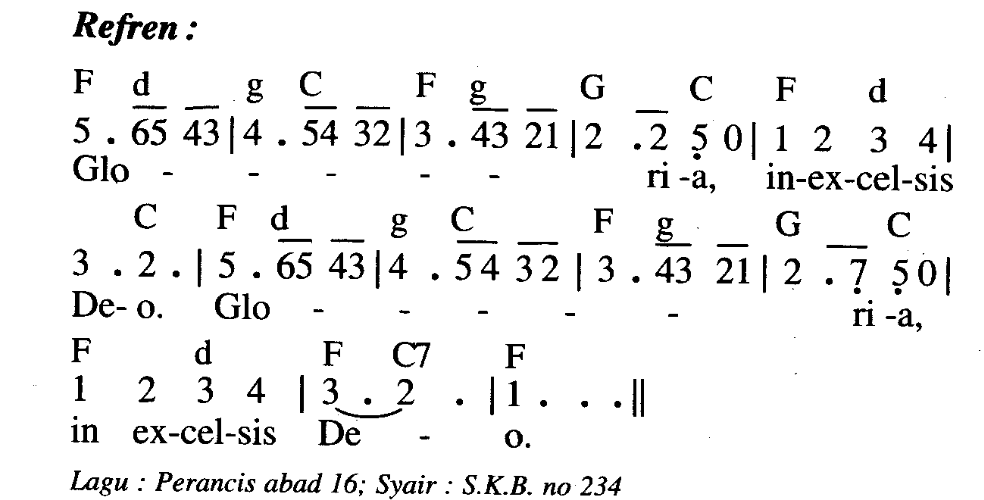
\includegraphics[scale=0.3]{mb334-gloria-b.png}

\newpage
\thispagestyle{empty}
\begin{center}
	
	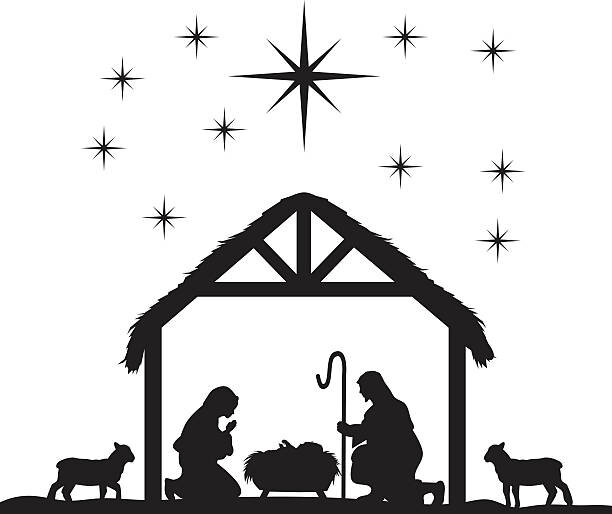
\includegraphics[scale=2]{manger.jpg}
	
	\Large
	
\vspace{2cm}
	
	Selamat Natal 2019\\dan\\Tahun Baru 2020
	
	\vspace{1cm}
	
	Semoga kita senantiasa dalam Berkat Tuhan
	
	\vspace{1cm}

	\textit{Berkah Dalem Gusti}
	
\end{center}
\end{document}